\let\negmedspace\undefined
\let\negthickspace\undefined
\documentclass[journal]{IEEEtran}
\usepackage[a5paper, margin=10mm, onecolumn]{geometry}
\usepackage{lmodern} % Ensure lmodern is loaded for pdflatex
\usepackage{tfrupee} % Include tfrupee package

\setlength{\headheight}{1cm} % Set the height of the header box
\setlength{\headsep}{0mm}  % Set the distance between the header box and the top of the text
\usepackage{romannum}
\usepackage{csquotes}
\usepackage{gvv-book}
\usepackage{gvv}
\usepackage{circuitikz}
\usepackage{cite}
\usepackage{float}
\usepackage{amsmath,amssymb,amsfonts,amsthm}
\usepackage{algorithmic}
\usepackage{graphicx}
\usepackage{textcomp}
\usepackage{xcolor}
\usepackage{txfonts}
\usepackage{listings}
\usepackage{enumitem}
\usepackage{mathtools}
\usepackage{gensymb}
\usepackage{comment}
\usepackage[breaklinks=true]{hyperref}
\usepackage{tkz-euclide} 
\usepackage{listings}
% \usepackage{gvv}                                        
\def\inputGnumericTable{}                                 
\usepackage[latin1]{inputenc}                                
\usepackage{color}                                            
\usepackage{array}                                            
\usepackage{longtable}                                       
\usepackage{calc}                                             
\usepackage{multirow} 
\usepackage{multicol}
\usepackage{hhline}   
\usepackage{enumitem}
\usepackage{ifthen}                                           
\usepackage{lscape}
\usepackage{caption}
\usepackage{tikz}
\usetikzlibrary{patterns}

\title{GATE 2017 Question Paper (Life Sciences - XL)}
\author{EE25BTECH11019 \\ Vivek Darji}
\date{}

\begin{document}

\maketitle
\section*{General Aptitude (GA)}
\section*{Q. 1 - Q. 5 carry one mark each.} 
\setcounter{enumi}{0}
\begin{enumerate}
    \item If $\brak{\rightarrow}$ denotes increasing order of intensity, then the meaning of the words $\brak{\text{walk} \rightarrow \text{jog} \rightarrow \text{sprint}}$ is analogous to $\brak{\text{bothered} \rightarrow \_ \rightarrow \text{daunted}}$. Which one of the given options is appropriate to fill the blank?\hfill $\brak{\text{GATE XL 2024}}$
    \begin{enumerate}
        \begin{multicols}{4}
            \item phased
            \item phrased
            \item fazed
            \item fused
        \end{multicols}
    \end{enumerate}

    \item Two wizards try to create a spell using all the four elements - water, air, fire, and earth. They decide to mix all these elements in all possible orders and work independently. After trying all possible combinations, they conclude the spell does not work. How many attempts does each wizard make before coming to this conclusion?\hfill $\brak{\text{GATE XL 2024}}$
    \begin{enumerate}
        \begin{multicols}{4}
            \item 24
            \item 48
            \item 16
            \item 12
        \end{multicols}
    \end{enumerate}

    \item In an engineering college of 10,000 students, 1,500 like neither their core branches nor other branches. The number of students who like their core branches is $\frac{1}{4}$th of the number of students who like other branches. The number of students who like both their core and other branches is 500. The number of students who like their core branches is\hfill $\brak{\text{GATE XL 2024}}$
    \begin{enumerate}
        \begin{multicols}{4}
            \item 1,800
            \item 3,500
            \item 1,600
            \item 1,500
        \end{multicols}
    \end{enumerate}

    \item For positive non-zero real variables $x$ and $y$, if
    \begin{align}
    \brak{x + \frac{1}{y}}^2 &= \brak{y + \frac{1}{x}}^2
    \end{align}
    then the value of $\frac{x}{y}$ is\hfill $\brak{\text{GATE XL 2024}}$
    \begin{enumerate}
        \begin{multicols}{4}
            \item 1
            \item $\frac{1}{2}$
            \item 2
            \item 4
        \end{multicols}
    \end{enumerate}

    \item In the sequence $6, 9, 14, x, 30, 41$, a possible value of $x$ is\hfill $\brak{\text{GATE XL 2024}}$
    \begin{enumerate}
        \begin{multicols}{4}
            \item 25
            \item 21
            \item 18
            \item 20
        \end{multicols}
    \end{enumerate}

\section*{Q. 6 - Q. 10 carry two mark each.} 
    \item Sequence the following sentences in a coherent passage:\hfill $\brak{\text{GATE XL 2024}}$
    \begin{enumerate}
        \begin{multicols}{4}
            \item QPSR
            \item QSPR
            \item SPRQ
            \item SATQ
        \end{multicols}
    \end{enumerate}

    \item A person sold two different items at the same price. He made $\brak{10\%}$ profit in one item, and $\brak{10\%}$ loss in the other item. In selling these two items, the person made a total of\hfill $\brak{\text{GATE XL 2024}}$
    \begin{enumerate}
        \begin{multicols}{4}
            \item \brak{1\%} profit
            \item \brak{2\%} profit
            \item \brak{1\%} loss
            \item \brak{2\%} loss
        \end{multicols}
    \end{enumerate}

    \item The pie charts depict the shares of various power generation technologies in the total electricity generation of a country for the years $2007$ and $2023$.

    \begin{figure}[H]
        \centering
        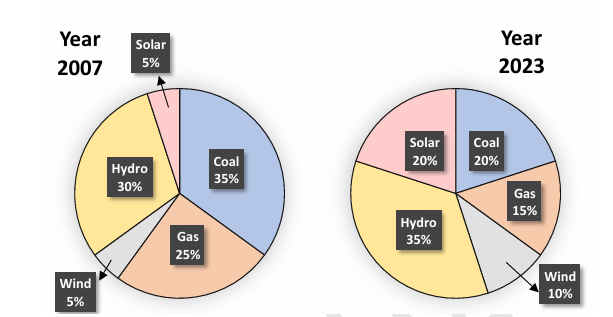
\includegraphics[width=0.8\columnwidth]{figs/xl2024_q8_que.png}
        \caption{Q8 que.}
    \end{figure}

    The renewable sources of electricity generation consist of Hydro, Solar and Wind. Assuming that the total electricity generated remains the same from $2007$ to $2023$, what is the percentage increase in the share of the renewable sources of electricity generation over this period?\hfill $\brak{\text{GATE XL 2024}}$

    \begin{enumerate}
        \begin{multicols}{4}
            \item $25\%$
            \item $50\%$
            \item $77.5\%$
            \item $62.5\%$
        \end{multicols}
    \end{enumerate}

    \item A cube is to be cut into 8 pieces of equal size and shape. Each cut should be straight and should not stop till it reaches the other end of the cube. The minimum number of such cuts required is\hfill $\brak{\text{GATE XL 2024}}$
    \begin{enumerate}
        \begin{multicols}{4}
            \item 3
            \item 4
            \item 7
            \item 8
        \end{multicols}
    \end{enumerate}

    \item In the $4 \times 4$ array shown below, each cell of the first three rows has either a cross $\brak{X}$ or a number.

    \begin{figure}[H]
        \centering
        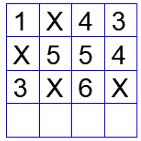
\includegraphics[width=0.5\columnwidth]{figs/xl2024_q10_que.png}
        \caption{Q10 que.}
    \end{figure}

    The number in a cell represents the count of the immediate neighboring cells $\brak{\text{left, right, top, bottom, diagonals}}$ NOT having a cross $\brak{X}$. Given that the last row has no crosses $\brak{X}$, the sum of the four numbers to be filled in the last row is\hfill $\brak{\text{GATE XL 2024}}$

    \begin{enumerate}
        \begin{multicols}{4}
            \item 11
            \item 10
            \item 12
            \item 9
        \end{multicols}
    \end{enumerate}

\maketitle
\section*{General Aptitude (GA)}
\section*{Q. 11 - Q. 19 carry one mark each.} 
\setcounter{enumi}{10}

    \item The CORRECT order of electronegativity is\hfill $\brak{\text{GATE XL 2024}}$
    \begin{enumerate}
        \begin{multicols}{2}
            \item Al $>$ Si $>$ P $>$ S
            \item Al $>$ S $>$ Si $>$ P
            \item S $>$ Si $>$ Al $>$ P
            \item S $>$ P $>$ Si $>$ Al
        \end{multicols}
    \end{enumerate}

    \item Which one of the following is the CORRECT representation of the variation of the Gibbs free energy $G$ of a substance with temperature $T$ at constant pressure?\hfill $\brak{\text{GATE XL 2024}}$
    \begin{enumerate}
            \item 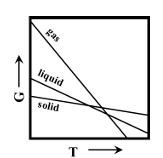
\includegraphics[width=0.2\columnwidth]{figs/xl2024_q12_op_A.png}
            \item 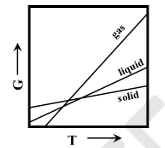
\includegraphics[width=0.2\columnwidth]{figs/xl2024_q12_op_B.png}
            \item 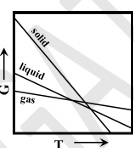
\includegraphics[width=0.2\columnwidth]{figs/xl2024_q12_op_C.png}
            \item 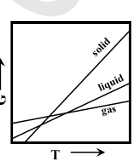
\includegraphics[width=0.2\columnwidth]{figs/xl2024_q12_op_D.png}
       
    \end{enumerate}

    \item Among the following, the structure representing histidine is\hfill $\brak{\text{GATE XL 2024}}$
    \begin{enumerate}
        
            \item 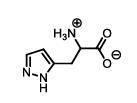
\includegraphics[width=0.2\columnwidth]{figs/xl2024_q13_op_A.png}
            \item 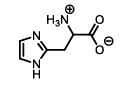
\includegraphics[width=0.2\columnwidth]{figs/xl2024_q13_op_B.png}
            \item 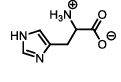
\includegraphics[width=0.2\columnwidth]{figs/xl2024_q13_op_C.png}
            \item 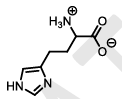
\includegraphics[width=0.2\columnwidth]{figs/xl2024_q13_op_D.png}
        
    \end{enumerate}

    \item The CORRECT order of acidity of the following compounds is:\hfill $\brak{\text{GATE XL 2024}}$
    \begin{figure}[H]
        \centering
        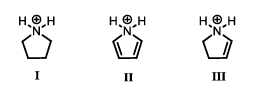
\includegraphics[width=0.5\columnwidth]{figs/xl2024_q14_que.png}
        \caption{Q14 que.}
    \end{figure}
    \begin{enumerate}
        \begin{multicols}{4}
            \item I $>$ II $>$ III
            \item II $>$ III $>$ I
            \item I $>$ III $>$ II
            \item III $>$ II $>$ I
        \end{multicols}
    \end{enumerate}

    \item The molecules A and B are a pair of:\hfill $\brak{\text{GATE XL 2024}}$
    \begin{figure}[H]
        \centering
        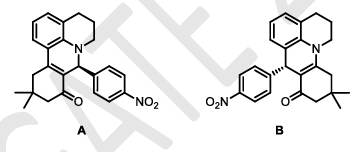
\includegraphics[width=0.5\columnwidth]{figs/xl2024_q15_que.png}
        \caption{Q15 que.}
    \end{figure}
    \begin{enumerate}
            \item enantiomers
            \item diastereomers
            \item conformational isomers
            \item constitutional isomers
    \end{enumerate}

    \item The CORRECT option(s) of Y for the following reaction is/are:\hfill $\brak{\text{GATE XL 2024}}$
    \begin{figure}[H]
        \centering
        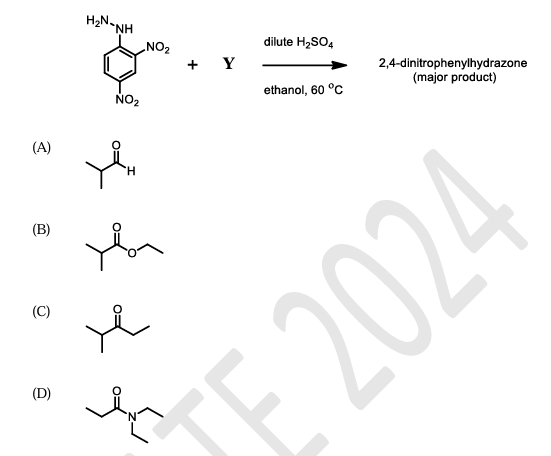
\includegraphics[width=0.8\columnwidth]{figs/xl2024_q16_que.png}
        \caption{Q16 que.}
    \end{figure}

    \item The maximum number of electrons that can be accommodated in the shell with $n = 2$ is (in integer).  
    (Given: $n$ = principal quantum number)\hfill $\brak{\text{GATE XL 2024}}$

    \item One mole of an ideal gas expands isothermally and reversibly to double its volume. If the expansion work done by the system is $1728.85$ J, the temperature of the system is K (rounded off to 2 decimal places).  
    (Given: Gas constant, $R = 8.314$ J K$^{-1}$ mol$^{-1}$)\hfill $\brak{\text{GATE XL 2024}}$

    \item The initial rate of a reaction triples when the concentration of a reactant, A, is doubled. The order of the reaction with respect to A is (rounded off to 2 decimal places).\hfill $\brak{\text{GATE XL 2024}}$
\section*{Q. 20 - Q. 27 carry two mark each.} 
    \item Each of the following alkenes undergoes addition reaction with bromine. Under the same reaction conditions, the CORRECT trend in the reaction rates is:\hfill $\brak{\text{GATE XL 2024}}$
    \begin{figure}[H]
        \centering
        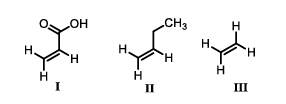
\includegraphics[width=0.9\columnwidth]{figs/xl2024_q20_que.png}
        \caption{Q20 que.}
    \end{figure}
    \begin{enumerate}
        \begin{multicols}{4}
            \item I $>$ II $>$ III
            \item II $>$ III $>$ I
            \item I $>$ III $>$ II
            \item III $>$ II $>$ I
        \end{multicols}
    \end{enumerate}

    \item An enzyme-catalyzed conversion of a substrate at $298$ K proceeds by a Michaelis-Menten mechanism. The Lineweaver-Burk plot for the analysis of the experimental data has an intercept along the $y$-axis of $0.357$ mmol$^{-1}$ dm$^3$ s and a slope of $2.10$ s. The CORRECT Michaelis constant for the reaction is (rounded off to $2$ decimal places).\hfill $\brak{\text{GATE XL 2024}}$
    \begin{enumerate}
            \item $5.88$ mmol dm$^{-3}$
            \item $5.88$ mmol dm$^{-3}$ s$^{-1}$
            \item $2.80$ mmol dm$^{-3}$
            \item $2.80$ mmol dm$^{-3}$ s$^{-1}$
    \end{enumerate}

    \item Which one among the following structures is the most stable conformer of $\brak{Z}$-pent-2-ene?\hfill $\brak{\text{GATE XL 2024}}$
    \begin{enumerate}
            \item 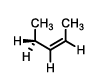
\includegraphics[width=0.2\columnwidth]{figs/xl2024_q22_op_A.png}
            \item 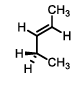
\includegraphics[width=0.2\columnwidth]{figs/xl2024_q22_op_B.png}
            \item 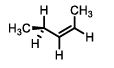
\includegraphics[width=0.2\columnwidth]{figs/xl2024_q22_op_C.png}
            \item 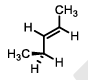
\includegraphics[width=0.2\columnwidth]{figs/xl2024_q22_op_D.png}
    \end{enumerate}

    \item Upon addition of compound $X$ to an aqueous AgNO$_3$ solution, a white precipitate appears instantly. Also, $X$ does not exhibit geometrical isomerism. The CORRECT option(s) for $X$ is/are:\hfill $\brak{\text{GATE XL 2024}}$
    \begin{enumerate}
        \begin{multicols}{2}
            \item $\brak{\text{[Cr(OH}_2)_4\text{Cl}_2\text{]Cl}}$
            \item $\brak{\text{[Cr(OH}_2)_5\text{Cl]Cl}_2}$
            \item $\brak{\text{[Cr(OH}_2)_6\text{]Cl}_3}$
            \item $\brak{\text{[Cr(OH}_2)_3\text{Cl}_3\text{]}}$
        \end{multicols}
    \end{enumerate}

    \item The paramagnetic species among the following is/are  
    (Given: Atomic numbers of Cr = $24$; Fe = $26$; Ni = $28$)\hfill $\brak{\text{GATE XL 2024}}$
    \begin{enumerate}
        \begin{multicols}{2}
            \item $\brak{\text{[Fe(CN)}_6\text{]}^{3-}}$
            \item $\brak{\text{[Ni(OH}_2)_6\text{]}^{2+}}$
            \item $\brak{\text{[Fe(CN)}_6\text{]}^{4-}}$
            \item $\brak{\text{[Cr(CN)}_6\text{]}^{3-}}$
        \end{multicols}
    \end{enumerate}

    \item The molecule(s) with non-zero dipole moment is/are:\hfill $\brak{\text{GATE XL 2024}}$
    \begin{enumerate}
        \begin{multicols}{4}
            \item N$_2$
            \item CO$_2$
            \item NO
            \item SO$_2$
        \end{multicols}
    \end{enumerate}

    \item The ionic product of water at $40\,^\circ$C is $2.92 \times 10^{-14}$ M$^2$. The pH of water at $40\,^\circ$C is\hfill $\brak{\text{GATE XL 2024}}$

    \item Given the standard reduction potentials $E^\circ$ for the half-cell reactions below, the standard Gibbs free energy of the dissolution of silver chloride in water, at $298$ K, is J mol$^{-1}$ (rounded off to nearest integer).  
    (Given: Faraday constant, $F = 96500$ C mol$^{-1}$; $J = C \times V$)  
    \begin{align}
    \text{AgCl(s)} + e^- &\rightarrow \text{Ag(s)} + \text{Cl}^-(aq); \quad E^\circ = 0.22\,\text{V} \\
    \text{Ag}^+(aq) + e^- &\rightarrow \text{Ag(s)}; \quad E^\circ = 0.80\,\text{V}
    \end{align}
    \hfill $\brak{\text{GATE XL 2024}}$

\maketitle
\section*{Biochemistry (XL-Q)}
\setcounter{enumi}{27}
\section*{Q.28 - Q.35 Carry ONE mark Each} 
    \item Which one of the following pairs of amino acids is NOT incorporated in a polypeptide chain?\hfill $\brak{\text{GATE XL 2024}}$
    \begin{enumerate}
            \item 4-Hydroxyproline and $\gamma$-carboxyglutamate
            \item $\gamma$-Carboxyglutamate and desmosine
            \item Ornithine and citrulline
            \item 4-Hydroxyproline and 5-hydroxylysine
    \end{enumerate}

    \item Mammalian cells cultured at low temperature $\brak{25 \text{ to } 30\,^\circ\text{C}}$ lead to an increased sterol content in the membrane. Elevated sterols in the membrane result in:\hfill $\brak{\text{GATE XL 2024}}$
    \begin{enumerate}
            \item an increase in membrane fluidity
            \item a decrease in membrane permeability to water
            \item an increase in membrane permeability to water
            \item a decrease in membrane fluidity
    \end{enumerate}

    \item Which one of the following metabolic intermediates is common to glycolysis, nucleotide synthesis and glycogen synthesis?\hfill $\brak{\text{GATE XL 2024}}$
    \begin{enumerate}
        \begin{multicols}{2}
            \item Citrate
            \item Oxaloacetate
            \item Glucose 6-phosphate
            \item Glycerol 3-phosphate
        \end{multicols}
    \end{enumerate}

    \item Cells that can give rise to all types of cells in the body are known as\hfill $\brak{\text{GATE XL 2024}}$
    \begin{enumerate}
        \begin{multicols}{2}
            \item totipotent stem cells
            \item pluripotent stem cells
            \item multipotent stem cells
            \item lymphoid progenitor cells
        \end{multicols}
    \end{enumerate}

    \item Which one or more of the following statements correctly describe(s) the addition of N-nucleotides during the rearrangement of the immunoglobulin heavy chain-encoding gene?\hfill $\brak{\text{GATE XL 2024}}$
    \begin{enumerate}
            \item Addition of N-nucleotides is template encoded.
            \item N-nucleotides are added by terminal deoxynucleotidyl transferase.
            \item The added N-nucleotides are common in V-D and D-J junction.
            \item N-nucleotides are added by the DNA polymerase II.
    \end{enumerate}

    \item A newly identified viral protein contains one long $\alpha$-helix spanning $60$ amino acid residues. The number of main chain H-bonds formed in this helix is (Answer in integer).\hfill $\brak{\text{GATE XL 2024}}$

    \item In a lactic acid solution at pH $4.8$, the concentrations of lactic acid and lactate are $0.01$ M and $0.087$ M, respectively. The calculated pKa of lactic acid is (Round off to one decimal place).\hfill $\brak{\text{GATE XL 2024}}$

    \item If a $10$ mM solution of a biomolecule in a cuvette of path length $10$ mm absorbs $90\%$ of the incident light at $280$ nm, the molar extinction coefficient of the biomolecule at this wavelength is M$^{-1}$cm$^{-1}$. (Round off to two decimal places)\hfill $\brak{\text{GATE XL 2024}}$

\section*{Q.36 - Q.46 Carry TWO mark Each}

    \item Metabolic intermediates provide the backbone for the synthesis of amino acids. Match the metabolic intermediates listed in Column I with their corresponding amino acids given in Column II.\hfill $\brak{\text{GATE XL 2024}}$
    \begin{multicols}{2}
    \noindent \textbf{Group I} \\
    P) $\alpha$-Ketoglutarate \\
    Q) Ribose 5-phosphate \\
    R) 3-Phosphoglycerate \\
    S) Phosphoenolpyruvate \\

    \columnbreak

    \noindent \textbf{Group II} \\
    1) Histidine \\
    2) Glutamate \\
    3) Aspartate \\
    4) Phenylalanine \\
    \end{multicols}

    \item Which one of the following is the correct match between the molecular properties listed in Column I and the corresponding biochemical separation methods in Column II?\hfill $\brak{\text{GATE XL 2024}}$
    \begin{multicols}{2}
    \noindent \textbf{Column I} \\
    P) Solubility \\
    Q) Ionic charge \\
    R) Polarity \\
    S) Molecular size \\

    \columnbreak

    \noindent \textbf{Column II} \\
    1) Reverse phase chromatography \\
    2) Ultracentrifugation \\
    3) Salting out \\
    4) Gel filtration \\
    \end{multicols}

    \item Which one or more of the following statements is/are correct regarding the electromotive force generated by electron transfer chain?\hfill $\brak{\text{GATE XL 2024}}$
    \begin{enumerate}
            \item It is used for the synthesis of ATP.
            \item It is not used for active transport process.
            \item It includes a pH gradient component.
            \item It does not include an electrical potential gradient component.
    \end{enumerate}

    \item Which one or more of the following statements is/are correct regarding the transport and retention of proteins in different cell organelles?\hfill $\brak{\text{GATE XL 2024}}$
    \begin{enumerate}
            \item Mannose 6-phosphate residues are involved in targeting proteins to lysosomes.
            \item Transport of proteins into the mitochondrial compartment is aided by positively charged amino acid residues at the N-terminus and internal hydrophobic segments.
            \item The retention of protein in the ER lumen requires the KDEL sequence motif at the C-terminus.
            \item Nuclear proteins are transported in an unfolded conformation and the nuclear localization signal sequence is subsequently cleaved by peptidases in the nucleoplasm.
    \end{enumerate}

    \item Which one or more of the following statements correctly describe(s) fluorescence spectroscopy?\hfill $\brak{\text{GATE XL 2024}}$
    \begin{enumerate}
            \item The emission maxima is independent of the excitation wavelength.
            \item The emission maxima depends on the concentration of a quencher.
            \item The emission maxima varies with solvent polarity.
            \item The emission maxima varies with temperature.
    \end{enumerate}

    \item Which one or more of the following statements is/are correct in the processing of pre-mRNA in eukaryotes?\hfill $\brak{\text{GATE XL 2024}}$
    \begin{enumerate}
        \item $3' \rightarrow 5'$ exonuclease activity is involved in the conversion of pre-mRNA to mRNA.
        \item $5'$-capping and addition of $3'$-poly A tail precedes splicing.
        \item Splicing of pre-mRNA occurs via transesterification reaction.
        \item Alternative splicing can yield different mRNA products from the same pre-mRNA.
    \end{enumerate}

    \item Which one or more of the following statements correctly describe(s) the changes upon the addition of puromycin during eukaryotic translation?\hfill $\brak{\text{GATE XL 2024}}$
    \begin{enumerate}
        \item Puromycin resembles aminoacyl end of the charged tRNA.
        \item Puromycin occupies the A site of the translating ribosomes.
        \item Puromycin occupies the P site of the translating ribosomes.
        \item Puromycin occupies the E site of the translating ribosomes.
    \end{enumerate}

    \item Factor H, a complement regulatory protein in plasma, binds C3b and\hfill $\brak{\text{GATE XL 2024}}$
    \begin{enumerate}
            \item competes with factor B to displace Bb from convertase.
            \item initiates the catabolism of C3b into inactivate products.
            \item then binds to C3bBb convertase.
            \item acts as a cofactor for factor I.
    \end{enumerate}

    \item The value of $V_{max}$ is (Round off to three decimal places)\hfill $\brak{\text{GATE XL 2024}}$

    \item A $5250$ base-pair long plasmid with $10$ negative supercoils would have a linking number of (Answer in integer).  
    (Considering $10.5$ base pairs per turn for B-DNA)\hfill $\brak{\text{GATE XL 2024}}$

    \item The spectrum of a protein obtained using electrospray ionization mass spectrometry (ESI-MS) is shown below. Two peaks, one at $m/z = 2960.6$ and the other at $m/z = 3552.5$, are marked. The mass of the protein associated with the $m/z = 2960.6$ peak is Da. (Round off to two decimal places)

    \begin{figure}[H]
        \centering
        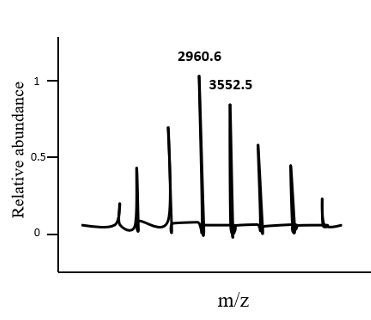
\includegraphics[width=0.5\columnwidth]{figs/xl2024_q46_que.png}
        \caption{Q46 que.}
    \end{figure}
    \hfill $\brak{\text{GATE XL 2024}}$

\maketitle
\section*{Botany (XL-R)}
\section*{Q. 47 - Q. 54 carry one mark each.} 
\setcounter{enumi}{46}
    \item Which one or more of the following statements is/are correct regarding the structure and function of immunoglobulin?\hfill $\brak{\text{GATE XL 2024}}$
    \begin{enumerate}
        \item The variable region of the heavy chain determines the class of immunoglobulin.
        \item The constant region of the heavy chain determines the class of immunoglobulin.
        \item The antigen binding site is formed by the variable regions of both heavy and light chains.
        \item The Fc region is responsible for antigen binding.
    \end{enumerate}

    \item Which one or more of the following statements is/are correct regarding the role of chaperones in protein folding?\hfill $\brak{\text{GATE XL 2024}}$
    \begin{enumerate}
        \item Chaperones prevent aggregation of unfolded proteins.
        \item Chaperones catalyze the formation of disulfide bonds.
        \item Chaperones assist in refolding of misfolded proteins.
        \item Chaperones are required for folding of all cytosolic proteins.
    \end{enumerate}

    \item Which one or more of the following statements is/are correct regarding the function of peroxisomes?\hfill $\brak{\text{GATE XL 2024}}$
    \begin{enumerate}
        \item Peroxisomes are involved in $\beta$-oxidation of very long chain fatty acids.
        \item Peroxisomes are involved in the synthesis of bile acids.
        \item Peroxisomes are involved in the detoxification of hydrogen peroxide.
        \item Peroxisomes are involved in the synthesis of cholesterol.
    \end{enumerate}

    \item Which one or more of the following statements is/are correct regarding the function of lysosomes?\hfill $\brak{\text{GATE XL 2024}}$
    \begin{enumerate}
        \item Lysosomes are involved in degradation of cellular waste.
        \item Lysosomes maintain acidic pH using proton pumps.
        \item Lysosomes are involved in synthesis of proteins.
        \item Lysosomes are involved in autophagy.
    \end{enumerate}

    \item Which of the following plant diseases is/are caused by nematode?\hfill $\brak{\text{GATE XL 2024}}$
    \begin{enumerate}
        \begin{multicols}{2}
            \item Cereal cyst of barley
            \item Ergot of rye
            \item Wart of potato
            \item Ear-cockle of wheat
        \end{multicols}
    \end{enumerate}

    \item Which of the following selectable marker genes is/are used for herbicide tolerance during genetic transformation of plants?\hfill $\brak{\text{GATE XL 2024}}$
    \begin{enumerate}
        \begin{multicols}{4}
            \item hpt
            \item bar
            \item nptII
            \item pmi
        \end{multicols}
    \end{enumerate}

    \item Which of the following statements is/are CORRECT with reference to rubber production from plants?\hfill $\brak{\text{GATE XL 2024}}$
    \begin{enumerate}
        \item Para rubber is produced from Hevea brasiliensis.
        \item India rubber is produced from Ficus elastica.
        \item Panama rubber is produced from Manihot glaziovii.
        \item Ceara rubber is produced from Castilla elastica.
    \end{enumerate}

\section*{Q. 55 - Q. 65 carry two mark each.} 
    \item In Calvin-Benson cycle, to produce $1$ molecule of glyceraldehyde 3-phosphate by fixing $3$ molecules of carbon dioxide, $9$ molecules of ATP and molecules (in integer) of NADPH are typically utilized.\hfill $\brak{\text{GATE XL 2024}}$

    \item In wild-type Arabidopsis thaliana, the four types of floral organs (sepal, petal, stamen, carpel) are arranged in concentric whorls from outside to inside. With reference to the ABC model of floral organ patterning, match the homeotic mutants in Group I with their respective arrangements of organs in the four whorls given in Group II.\hfill $\brak{\text{GATE XL 2024}}$
    \begin{multicols}{2}
    \noindent \textbf{Group I} \\
    P) A class mutants \\
    Q) B class mutants \\
    R) C class mutants \\

    \columnbreak

    \noindent \textbf{Group II} \\
    1) sepal, sepal, carpel, carpel \\
    2) sepal, petal, petal, sepal \\
    3) carpel, stamen, stamen, carpel \\
    \end{multicols}

    \item Match the inhibitors in Group I with their respective targets in Group II.\hfill $\brak{\text{GATE XL 2024}}$
    \begin{multicols}{2}
    \noindent \textbf{Group I} \\
    P) Oligomycin \\
    Q) Antimycin A \\
    R) DCMU \\
    S) Valinomycin \\

    \columnbreak

    \noindent \textbf{Group II} \\
    1) Cytochrome bc$_1$ complex \\
    2) Photosystem II \\
    3) K$^+$ ionophore \\
    4) F$_0$ ATP synthase \\
    \end{multicols}

    \item With reference to Agrobacterium tumefaciens-mediated plant transformation, match the virulence factors in Group I with their protein types in Group II.\hfill $\brak{\text{GATE XL 2024}}$
    \begin{multicols}{2}
    \noindent \textbf{Group I} \\
    P) VirG \\
    Q) VirA \\
    R) VirE \\
    S) VirC \\

    \columnbreak

    \noindent \textbf{Group II} \\
    1) Kinase \\
    2) Helicase \\
    3) Transcriptional activator \\
    4) - \\
    \end{multicols}

    \item Match the plant products in Group I with the plant species in Group II that produce them and the respective plant parts in Group III where they accumulate the most.\hfill $\brak{\text{GATE XL 2024}}$
    \begin{multicols}{3}
    \noindent \textbf{Group I} \\
    P) Liquorice \\
    Q) Quinine \\
    R) Henna \\
    S) Saffron \\

    \columnbreak

    \noindent \textbf{Group II} \\
    1) Cinchona calisaya \\
    2) Lawsonia inermis \\
    3) Glycyrrhiza glabra \\
    4) Crocus sativus \\

    \columnbreak

    \noindent \textbf{Group III} \\
    a) Leaf \\
    b) Root \\
    c) Flower \\
    d) Bark \\
    e) Seed \\
    \end{multicols}

    \item Match the types of ecological interactions in Group I with their respective definitions in Group II.\hfill $\brak{\text{GATE XL 2024}}$
    \begin{multicols}{2}
    \noindent \textbf{Group I} \\
    P) Protocooperation \\
    Q) Commensalism \\
    R) Amensalism \\
    S) Helotism \\

    \columnbreak

    \noindent \textbf{Group II} \\
    1) One species is harmed but the other is neither harmed nor benefitted \\
    2) A type of mutualism where one species is benefitted more than the other \\
    3) Both species are benefitted but the interaction is not obligatory \\
    4) One species is benefitted without harming the other \\
    \end{multicols}

    \item Match the types of ecological energy productivity in Group I with their respective definitions in Group II.\hfill $\brak{\text{GATE XL 2024}}$
    \begin{multicols}{2}
    \noindent \textbf{Group I} \\
    P) Net primary productivity \\
    Q) Gross primary productivity \\
    R) Net productivity \\
    S) Secondary productivity \\

    \columnbreak

    \noindent \textbf{Group II} \\
    1) Total amount of energy produced by autotrophs \\
    2) Amount of energy stored by autotrophs after respiration \\
    3) Net gain of energy by the consumers after energy loss \\
    4) Unused amount of energy after - \\
    \end{multicols}

    \item Which of the following combinations of plant diseases and the types of their causal organisms is/are CORRECT?\hfill $\brak{\text{GATE XL 2024}}$
    \begin{enumerate}
        \item Late blight of potato - Bacteria
        \item Black rot of crucifer - Bacteria
        \item Tungro disease of rice - Mycoplasma
        \item Root knot of tomato - Nematode
    \end{enumerate}

    \item Identify the CORRECT combination(s) of plant natural products and the categories they belong to.\hfill $\brak{\text{GATE XL 2024}}$
    \begin{enumerate}
        \begin{multicols}{2}
            \item Dhurrin - Phenolic compounds
            \item Farnesene - Terpenoids
            \item Naringenin - Cyanogenic glycosides
            \item Vincristine - Alkaloids
        \end{multicols}
    \end{enumerate}

    \item Identify the CORRECT combination(s) between the enzymes in Group I and the reactions in Group II they catalyze.\hfill $\brak{\text{GATE XL 2024}}$
    \begin{multicols}{2}
    \noindent \textbf{Group I} \\
    P) Cinnamate-4-hydroxylase \\
    Q) Glycerate kinase \\
    R) PEP carboxylase \\
    S) Nitrate reductase \\

    \columnbreak

    \noindent \textbf{Group II} \\
    1) L-phenylalanine $\rightarrow$ Cinnamic acid \\
    2) Glyceraldehyde 3-phosphate $\rightarrow$ dihydroxyacetone phosphate \\
    3) Glycolate + O$_2$ $\rightarrow$ Glyoxylate + H$_2$O$_2$ \\
    4) NO$_3^-$ + NAD(P)H + H$^+$ $\rightarrow$ NO$_2^-$ + NAD(P)$^+$ + H$_2$O \\
    \end{multicols}

    \item In a genetic cross between two pure-line parents differing in the two independently segregating traits, plant height $\brak{\text{tall vs dwarf}}$ and flower color $\brak{\text{purple vs white}}$, all the F$_1$ plants were tall with purple flowers. In a testcross population involving these F$_1$ individuals, the expected percentage $\brak{\%}$ of dwarf plants with purple flower would be (in integer).\hfill $\brak{\text{GATE XL 2024}}$

    \item The mRNA of a hypothetical plant gene HSDU is $800$-nucleotide long and encodes a protein of $160$ amino acid residues. The calculated length of HSDU CDS would be nucleotides (in integer).\hfill $\brak{\text{GATE XL 2024}}$

\maketitle
\section*{Botany (XL-R)}
\section*{Q. 66 - Q. 73 carry one mark each.} 
\setcounter{enumi}{65}
    \item Which one of the following bacterial species can cause atypical pneumonia?\hfill $\brak{\text{GATE XL 2024}}$
    \begin{enumerate}
        \begin{multicols}{2}
            \item Chlamydia pneumoniae
            \item Streptococcus pneumoniae
            \item Klebsiella pneumoniae
            \item Haemophilus influenzae
        \end{multicols}
    \end{enumerate}

    \item Which one of the following organisms has axial filaments?\hfill $\brak{\text{GATE XL 2024}}$
    \begin{enumerate}
        \begin{multicols}{2}
            \item Mycobacterium tuberculosis
            \item Pasteurella multocida
            \item Treponema pallidum
            \item Shigella dysenteriae
        \end{multicols}
    \end{enumerate}

    \item Who among the following scientists was the pioneer in development of chemotherapy?\hfill $\brak{\text{GATE XL 2024}}$
    \begin{enumerate}
        \begin{multicols}{4}
            \item Elie Metchnikoff
            \item Robert Koch
            \item Paul Ehrlich
            \item Ronald Ross
        \end{multicols}
    \end{enumerate}

    \item In which of the following processes is glutaraldehyde used as a sterilizing agent?\hfill $\brak{\text{GATE XL 2024}}$
    \begin{enumerate}
        \begin{multicols}{4}
            \item Pasteurization
            \item Incineration
            \item Cold sterilization
            \item Autoclaving
        \end{multicols}
    \end{enumerate}

    \item The most abundant class of immunoglobulins in serum is\hfill $\brak{\text{GATE XL 2024}}$
    \begin{enumerate}
        \begin{multicols}{4}
            \item IgM
            \item IgA
            \item IgD
            \item IgG
        \end{multicols}
    \end{enumerate}

    \item Which one of the following double-stranded sequences will NOT be recognized by a Type IIP restriction endonuclease?\hfill $\brak{\text{GATE XL 2024}}$
    \begin{enumerate}
        \item 5' -- GGTACC -- 3' \quad 3' -- CCTAGG -- 5'
        \item 5' -- GGATCC -- 3' \quad 3' -- CCTAGG -- 5'
        \item 5' -- CATATG -- 3' \quad 3' -- GTATAC -- 5'
        \item 5' -- GATTTC -- 3' \quad 3' -- CTAAAG -- 5'
    \end{enumerate}

    \item Which one of the following uses inorganic compounds as an energy source?\hfill $\brak{\text{GATE XL 2024}}$
    \begin{enumerate}
        \begin{multicols}{2}
            \item Heterotrophs
            \item Chemolithotrophs
            \item Chemoorganotrophs
            \item Photoheterotrophs
        \end{multicols}
    \end{enumerate}

    \item Which one of the following represents the abundance of the organisms found in soil?\hfill $\brak{\text{GATE XL 2024}}$
    \begin{enumerate}
        \item Fungi $>$ Aerobic bacteria $>$ Anaerobic bacteria
        \item Aerobic bacteria $>$ Fungi $>$ Anaerobic bacteria
        \item Anaerobic bacteria $>$ Aerobic bacteria $>$ Fungi
        \item Aerobic bacteria $>$ Anaerobic bacteria $>$ Fungi
    \end{enumerate}
\section*{Q.74 - Q. 84 carry two mark each.} 
    \item Match the antibiotics in Group I with the microorganisms that produce them in Group II.\hfill $\brak{\text{GATE XL 2024}}$
    \begin{multicols}{2}
    \noindent \textbf{Group I} \\
    P) Streptomycin \\
    Q) Bacitracin \\
    R) Amphotericin B \\
    S) Chloramphenicol \\

    \columnbreak

    \noindent \textbf{Group II} \\
    1) Streptomyces griseus \\
    2) Bacillus licheniformis \\
    3) Streptomyces venezuelae \\
    4) Streptomyces nodosus \\
    \end{multicols}

    \item Which one of the following redox couples has the highest tendency to donate electrons?\hfill $\brak{\text{GATE XL 2024}}$
    \begin{enumerate}
        \begin{multicols}{2}
            \item Fumarate / succinate 
            \item NAD$^+$/NADH
            \item FAD/FADH
            \item Pyruvate/lactate
        \end{multicols}
    \end{enumerate}

    \item Which of the following is/are active transport mechanism(s) in prokaryotes where the substance is chemically altered during transport across the membrane?\hfill $\brak{\text{GATE XL 2024}}$
    \begin{enumerate}
        \begin{multicols}{2}
            \item Group translocation
            \item Simple diffusion
            \item Facilitated diffusion
            \item Osmosis
        \end{multicols}
    \end{enumerate}

    \item Which of the following cocci is/are examples of division in one plane?\hfill $\brak{\text{GATE XL 2024}}$
    \begin{enumerate}
        \begin{multicols}{4}
            \item Staphylococci
            \item Streptococci
            \item Micrococci
            \item Diplococci
        \end{multicols}
    \end{enumerate}

    \item Which of the following event(s) occur(s) during translation in prokaryotes?\hfill $\brak{\text{GATE XL 2024}}$
    \begin{enumerate}
        \item tRNA binding to the start codon of mRNA on the $30$S subunit of ribosome
        \item Anticodon of tRNA binding to the start codon of mRNA on the $50$S subunit of ribosome
        \item The ribosome continues to move along the mRNA to add new amino acids to the polypeptide
        \item The polypeptide is released when the ribosome reaches the stop codon
    \end{enumerate}

    \item Which of the following is/are consequence(s) of nitrous acid $\brak{\text{HNO}_2}$ mediated deamination?\hfill $\brak{\text{GATE XL 2024}}$
    \begin{enumerate}
        \item Conversion of cytosine to uracil
        \item Conversion of adenine to hypoxanthine
        \item Conversion of guanine to xanthine
        \item Addition of alkyl group to the bases
    \end{enumerate}

    \item At root nodules, which of the following C$_4$ organic acid(s) is/are transported across the symbiosome membrane and into bacteroids?\hfill $\brak{\text{GATE XL 2024}}$
    \begin{enumerate}
        \begin{multicols}{4}
            \item Succinate
            \item Pyruvate
            \item Malate
            \item Fumarate
        \end{multicols}
    \end{enumerate}

    \item Which of the following is/are TRUE about the Escherichia coli chromosome?\hfill $\brak{\text{GATE XL 2024}}$
    \begin{enumerate}
        \item It is typically bound by histones.
        \item It is circular in nature.
        \item It contains multiple origins of replication.
        \item It is linear and segmented.
    \end{enumerate}

    \item At $t = 0$, the bacterial cell number is $10{,}000$ cells/mL. At $t = 480$ minutes, the cell number increased to $320{,}000$ cells/mL. The mean generation time during this exponential growth period, rounded off to the nearest integer, is minutes.\hfill $\brak{\text{GATE XL 2024}}$

    \item A landfill sample was analyzed by dilution and plating techniques for viable bacterial count. When one gram of the landfill sample was diluted $1 \times 10^{-4}$ $\brak{\text{w/v}}$, it yielded $400$ CFU. The viable bacterial count $\brak{\text{in million, rounded off to the nearest integer}}$ in one gram landfill sample is\hfill $\brak{\text{GATE XL 2024}}$

    \item A fluorescence microscope with an objective lens of numerical aperture $\brak{\text{NA}} = 1.5$ is used with light of wavelength $\lambda = 600$ nanometers. The lateral resolution limit of this microscope, rounded off to the nearest integer, is nanometers.\hfill $\brak{\text{GATE XL 2024}}$

\maketitle
\section*{Zoology (XL-T)}
\section*{Q. 85 - Q. 92 carry one mark each.} 
\setcounter{enumi}{84}
    \item Which one of the following statements about gene expression is INCORRECT?\hfill $\brak{\text{GATE XL 2024}}$
    \begin{enumerate}
        \begin{multicols}{2}
            \item DNA is transcribed to mRNA.
            \item mRNA can be reverse-transcribed to DNA.
            \item mRNA can be translated to protein.
            \item Protein can be reverse-translated to mRNA.
        \end{multicols}
    \end{enumerate}

    \item Which one of the following tissues/organs is least likely to experience graft rejection when transplanted from a person to an unrelated person?\hfill $\brak{\text{GATE XL 2024}}$
    \begin{enumerate}
        \begin{multicols}{4}
            \item Bone marrow
            \item Cornea
            \item Heart
            \item Kidney
        \end{multicols}
    \end{enumerate}

    \item Codon bias is correlated with the relative frequencies of which one of the following types of RNA?\hfill $\brak{\text{GATE XL 2024}}$
    \begin{enumerate}
        \begin{multicols}{4}
            \item mRNA
            \item rRNA
            \item siRNA
            \item tRNA
        \end{multicols}
    \end{enumerate}

    \item CREB1 is a eukaryotic transcription factor. In which one of the following compartments of the cell is CREB1 predominantly localized?\hfill $\brak{\text{GATE XL 2024}}$
    \begin{enumerate}
        \begin{multicols}{4}
            \item Lysosomes
            \item Mitochondria
            \item Nucleus
            \item Peroxisomes
        \end{multicols}
    \end{enumerate}

    \item In certain species of salamanders, male-female pairs have multiple mating partners in a breeding season. Which one of the following terminologies accurately describes this mating system?\hfill $\brak{\text{GATE XL 2024}}$
    \begin{enumerate}
        \begin{multicols}{4}
            \item Monogamy
            \item Polyandry
            \item Polygyny
            \item Polygynandry
        \end{multicols}
    \end{enumerate}

    \item Which one of the following statements describes the key function of human sweat glands?\hfill $\brak{\text{GATE XL 2024}}$
    \begin{enumerate}
        \begin{multicols}{2}
            \item They serve as touch sensors.
            \item They secrete hormones.
            \item They regulate body temperature.
            \item They store fat.
        \end{multicols}
    \end{enumerate}

    \item Urease enzyme catalyzes the conversion of urea into ammonia and carbon dioxide. Which one of the following organisms expresses urease enzyme?\hfill $\brak{\text{GATE XL 2024}}$
    \begin{enumerate}
        \begin{multicols}{2}
            \item Caenorhabditis elegans
            \item Drosophila melanogaster
            \item Helicobacter pylori
            \item Homo sapiens
        \end{multicols}
    \end{enumerate}

    \item The human genetic code is triplet in nature with $64$ codons made using four nucleotides. If the human genetic code was doublet in nature, the number of codons theoretically possible from four nucleotides is (Answer in integer).\hfill $\brak{\text{GATE XL 2024}}$

\section*{Q. 93 - Q. 103 carry two mark each.} 
    \item Which one of the following statements is NOT TRUE of glycosaminoglycans?\hfill $\brak{\text{GATE XL 2024}}$
    \begin{enumerate}
        \item Glycosaminoglycans are composed of repeating disaccharide units.
        \item Glycosaminoglycans consist of amino sugars that are frequently sulfated.
        \item Hyaluronic acid is an example of a glycosaminoglycan.
        \item Methionine is the predominant amino acid to which glycosaminoglycan chains are conjugated to form proteoglycans.
    \end{enumerate}

    \item Which one of the options correctly matches the human tissues/organs with their embryonic germ layers of origin?\hfill $\brak{\text{GATE XL 2024}}$
    \begin{multicols}{2}
    \noindent \textbf{Tissues/organs} \\
    P) Liver \\
    Q) Cerebellum \\
    R) Femur \\

    \columnbreak

    \noindent \textbf{Embryonic germ layers} \\
    I) Ectoderm \\
    II) Endoderm \\
    III) Mesoderm \\
    \end{multicols}

    \item Consider a large population of a finch species, where both small and big beak sizes are advantageous, and an intermediate beak size is maladaptive. Over a period of $10$ years, which one of the following evolutionary processes is most likely to operate on the beak size of this finch population?\hfill $\brak{\text{GATE XL 2024}}$
    \begin{enumerate}
        \begin{multicols}{2}
            \item Directional selection
            \item Disruptive selection
            \item Genetic drift
            \item Stabilizing selection
        \end{multicols}
    \end{enumerate}

    \item When the blood glucose level of a healthy person is $100$ mg/dL, which one of the following options is most likely to represent the level of glucose in the urine of that person?\hfill $\brak{\text{GATE XL 2024}}$
    \begin{enumerate}
        \begin{multicols}{4}
            \item $< 1$ mg/dL
            \item $10$ mg/dL
            \item $50$ mg/dL
            \item $100$ mg/dL
        \end{multicols}
    \end{enumerate}

    \item Which one of the following rooted tree topologies best describes the primate phylogeny?\hfill $\brak{\text{GATE XL 2024}}$
    \begin{figure}[H]
        \centering
        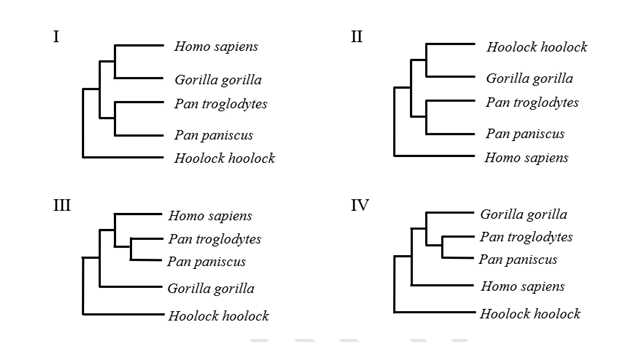
\includegraphics[width=0.8\columnwidth]{figs/xl2024_q97_que.png}
        \caption{Q97 que.}
    \end{figure}
    \begin{enumerate}
        \begin{multicols}{4}
            \item I
            \item II
            \item III
            \item IV
        \end{multicols}
    \end{enumerate}

    \item Consider a species of brightly colored beetle. Which one or more of the following observations suggest(s) that this species is aposematic?\hfill $\brak{\text{GATE XL 2024}}$
    \begin{enumerate}
        \item Both male and female beetles are brightly colored.
        \item Only male beetles are brightly colored.
        \item Only female beetles are brightly colored.
        \item The beetle species is toxic and distasteful.
    \end{enumerate}

    \item The embryos of which one or more of the following animals show meroblastic cleavage?\hfill $\brak{\text{GATE XL 2024}}$
    \begin{enumerate}
            \item Danio rerio $\brak{\text{zebrafish}}$
            \item Gallus gallus $\brak{\text{chicken}}$
            \item Synapta digita $\brak{\text{sea cucumber}}$
            \item Xenopus laevis $\brak{\text{frog}}$
    \end{enumerate}

    \item Which one or more of the following parasites is/are typically transmitted by mosquitoes as vector?\hfill $\brak{\text{GATE XL 2024}}$
    \begin{enumerate}
        \begin{multicols}{2}
            \item Leishmania donovani
            \item Plasmodium vivax
            \item Wuchereria bancrofti
            \item Trichuris trichiura
        \end{multicols}
    \end{enumerate}

    \item Consider the following nucleotide sequence:  \\
    $5'$-GCCGCCAUGGCGUCUGCUAGCUGGCUCGAUCGCGAGCGAUCGUACGU\\AUAGUAUGAA-$3'$  
    Assume canonical initiation, canonical termination, no post-translational modification, and the average molecular mass of an amino acid to be $110$ daltons.  
    The theoretical molecular mass of the polypeptide translated from the above nucleotide sequence is daltons. (Answer in integer)\hfill $\brak{\text{GATE XL 2024}}$

    \item The pKa of a buffer solution with pH of $5$, consisting of $0.4$ M sodium acetate and $0.04$ M acetic acid, is (Answer in integer).\hfill $\brak{\text{GATE XL 2024}}$

    \item Consider a healthy person with the following lung volumes:  
    Residual volume $= 900$ mL  
    Expiratory reserve volume $= 800$ mL  
    Tidal volume $= 200$ mL  
    If the total lung capacity is $5500$ mL, then the inspiratory reserve volume of the person is mL. (Answer in integer)\hfill $\brak{\text{GATE XL 2024}}$

\maketitle
\section*{Food Technology (XL-U)}
\section*{Q. 104 - Q. 111 carry one mark each.} 
\setcounter{enumi}{103}
    \item Which one of the following fungi produces aflatoxins?\hfill $\brak{\text{GATE XL 2024}}$
    \begin{enumerate}
        \begin{multicols}{2}
            \item Aspergillus niger
            \item Fusarium verticillioides
            \item Aspergillus flavus
            \item Rhizopus oligosporus
        \end{multicols}
    \end{enumerate}

    \item Under standard conditions in animal feeding studies, the weight gained $\brak{\text{in grams}}$ per gram of protein consumed by an animal is termed as:\hfill $\brak{\text{GATE XL 2024}}$
    \begin{enumerate}
        \begin{multicols}{2}
            \item Net Protein Ratio
            \item Net Protein Utilization
            \item Coefficient of Protein Digestibility
            \item Protein Efficiency Ratio
        \end{multicols}
    \end{enumerate}

    \item Xerophthalmia is caused due to the deficiency of:\hfill $\brak{\text{GATE XL 2024}}$
    \begin{enumerate}
        \begin{multicols}{4}
            \item Thiamin
            \item Pantothenic acid
            \item Vitamin A
            \item Vitamin C
        \end{multicols}
    \end{enumerate}

    \item Which one of the following steps is used to remove phosphatides from crude oil in the refining process?\hfill $\brak{\text{GATE XL 2024}}$
    \begin{enumerate}
        \begin{multicols}{4}
            \item Neutralization
            \item Bleaching
            \item Degumming
            \item Deodorization
        \end{multicols}
    \end{enumerate}

    \item The unique flavor of chocolate and cocoa is due to the formation of:\hfill $\brak{\text{GATE XL 2024}}$
    \begin{enumerate}
        \begin{multicols}{2}
            \item 5-methyl-2-phenyl-2-hexenal
            \item Cyclotene
            \item Furaneol
            \item Maltol
        \end{multicols}
    \end{enumerate}

    \item Which one of the following statements regarding Hazard Analysis Critical Control Point $\brak{\text{HACCP}}$ plan is NOT correct?\hfill $\brak{\text{GATE XL 2024}}$
    \begin{enumerate}
        \item HACCP is a management tool for ensuring food safety.
        \item HACCP involves five preliminary steps and seven principles.
        \item HACCP is not effective without prior implementation of prerequisite programs.
        \item HACCP plan involves establishment of corrective actions as second principle.
    \end{enumerate}

    \item The product of cabbage fermentation by *Leuconostoc mesenteroides* is:\hfill $\brak{\text{GATE XL 2024}}$
    \begin{enumerate}
        \begin{multicols}{4}
            \item Tempeh
            \item Natto
            \item Sauerkraut
            \item Miso
        \end{multicols}
    \end{enumerate}

    \item Which one of the following absorbents is NOT used as an ethylene absorber in active packaging of fruits and vegetables?\hfill $\brak{\text{GATE XL 2024}}$
    \begin{enumerate}
        \begin{multicols}{2}
            \item Potassium permanganate
            \item Activated carbon
            \item Calcium hydroxide
            \item Silica gel
        \end{multicols}
    \end{enumerate}
\section*{Q.112 - Q.122 carry two mark each.} 
    \item Which one of the following statements regarding moisture sorption isotherms of a dried food is NOT correct?\hfill $\brak{\text{GATE XL 2024}}$
    \begin{enumerate}
        \item At a given temperature, the difference between adsorption and desorption moisture isotherms is known as hysteresis.
        \item At a given temperature and water activity, an adsorption isotherm exhibits higher equilibrium moisture content than a desorption isotherm in hysteresis.
        \item At a given moisture content, effect of temperature on a moisture sorption isotherm follows the Clausius-Clapeyron equation.
        \item The Guggenheim-Anderson-de Boer $\brak{\text{GAB}}$ equation is a multilayer moisture sorption model.
    \end{enumerate}

    \item Processing of fluid milk at $72\,^\circ$C for $15$ seconds is termed as:\hfill $\brak{\text{GATE XL 2024}}$
    \begin{enumerate}
            \item High-temperature, short-time $\brak{\text{HTST}}$ pasteurization
            \item Low-temperature, long-time $\brak{\text{LTLT}}$ pasteurization
            \item Ultra high-temperature $\brak{\text{UHT}}$ pasteurization
            \item Homogenization process
    \end{enumerate}

    \item Match the anti-nutritional factors in Column I with their corresponding activity given in Column II.\hfill $\brak{\text{GATE XL 2024}}$
    \begin{multicols}{2}
    \noindent \textbf{Column I} \\
    P) Lectin \\
    Q) Stachyose \\
    R) Phytate \\
    S) Knuitz type inhibitor \\

    \columnbreak

    \noindent \textbf{Column II} \\
    1) Flatulence \\
    2) Chelates with divalent cations and reduces their bioavailability \\
    3) Inhibits trypsin and chymotrypsin \\
    4) Hemagglutination \\
    \end{multicols}

    \item Which of the following fatty acids is/are known to increase the low-density lipoprotein $\brak{\text{LDL}}$ levels?\hfill $\brak{\text{GATE XL 2024}}$
    \begin{enumerate}
        \begin{multicols}{2}
            \item Omega-3 fatty acids
            \item Trans fatty acids
            \item Conjugated linoleic acids
            \item Saturated fatty acids
        \end{multicols}
    \end{enumerate}

    \item The addition of which of the following to high-methoxyl pectin will result in gel formation?\hfill $\brak{\text{GATE XL 2024}}$
    \begin{enumerate}
        \begin{multicols}{4}
            \item Calcium ions
            \item Hydrogen ions
            \item Sodium ions
            \item Sugar
        \end{multicols}
    \end{enumerate}

    \item Which of the following steps in food processing is/are used to reduce acrylamide formation in food products?\hfill $\brak{\text{GATE XL 2024}}$
    \begin{enumerate}
        \item Pretreatment using asparaginase
        \item Lowering the pH
        \item Increasing the temperature
        \item Adding glucose
    \end{enumerate}

    \item Which of the following enzymes is/are used for the production of high fructose syrup $\brak{\text{HFS}}$ from corn starch?\hfill $\brak{\text{GATE XL 2024}}$
    \begin{enumerate}
        \begin{multicols}{4}
            \item $\alpha$-Amylase
            \item $\beta$-Amylase
            \item Xylose isomerase
            \item Glucoamylase
        \end{multicols}
    \end{enumerate}

    \item Which of the following is/are typical characteristic(s) of a fungal cell?\hfill $\brak{\text{GATE XL 2024}}$
    \begin{enumerate}
        \item Presence of histone proteins
        \item Presence of peptidoglycans in the cell wall
        \item Presence of chitin in the cell wall
        \item Presence of pseudomurein in the cell wall
    \end{enumerate}

    \item Which of the following statements is/are correct regarding food and water borne diseases and the class of causative microorganisms?\hfill $\brak{\text{GATE XL 2024}}$
    \begin{enumerate}
        \item Legionellosis is a bacterial disease.
        \item Giardiasis is caused by protists.
        \item Typhoid fever is caused by virus.
        \item Listeriosis is a fungal disease.
    \end{enumerate}

    \item Which of the following statements is/are true?\hfill $\brak{\text{GATE XL 2024}}$
    \begin{enumerate}
        \item Hagen-Poiseuille's law is used for calculation of molecular diffusion.
        \item Fick's law is used for calculation of energy requirement in size reduction.
        \item Rittinger's law is used for calculation of energy requirement in size reduction.
        \item Stokes' law is used for calculation of terminal velocity.
    \end{enumerate}

    \item A $10$ kg tomato pulp is concentrated from an initial moisture content of $90\%$ $\brak{\text{wet weight basis}}$ to $35\%$ $\brak{\text{wet weight basis}}$. The weight of the concentrate in kg is (round off to $2$ decimal places).\hfill $\brak{\text{GATE XL 2024}}$
\end{enumerate}
\end{document}